\documentclass[11pt,a4paper]{article}

% ===================== PAQUETES =====================
\usepackage[utf8]{inputenc}
\usepackage[T1]{fontenc}
\usepackage[spanish,es-tabla]{babel}
\usepackage[margin=2.5cm]{geometry}
\usepackage{booktabs}
\usepackage{array}
\usepackage{caption}
\usepackage{graphicx}
\usepackage{xcolor}
\usepackage{hyperref}
\usepackage{enumitem}
\usepackage{fancyhdr}

\graphicspath{{img/}}

\hypersetup{
  colorlinks=true,
  linkcolor=black,
  urlcolor=blue!50!black,
  citecolor=blue!50!black,
  pdftitle={Laboratorio - Comprension de datos de la extraccion de la pesca},
  pdfauthor={Grupo}
}

\captionsetup{font=small,labelfont=bf}

% ===================== ENCABEZADO =====================
\pagestyle{fancy}
\fancyhf{}
\fancyhead[L]{Minería de Datos - Comprensión de datos}
\fancyhead[R]{Extracción de la pesca}
\fancyfoot[C]{\thepage}
\renewcommand{\headrulewidth}{0.4pt}

\setlist[itemize]{topsep=2pt,itemsep=2pt}

\begin{document}

% ===================================================================
% CARATULA
% ===================================================================
\begin{titlepage}
\thispagestyle{empty}
\begin{center}

{\LARGE \textbf{UNIVERSIDAD NACIONAL MAYOR DE SAN MARCOS}}\\[3pt]
{\itshape\small Decana de América, fundada en 1551}\\[40pt]

% El logo es opcional: si el archivo no existe en img/, el informe compila igual.
\IfFileExists{img/logo_unmsm_0.png}{\includegraphics[width=3.2cm]{img/logo_unmsm_0.png}\\[40pt]}{\vspace{60pt}}

{\large \textbf{FACULTAD DE INGENIERÍA DE SISTEMA E INFORMÁTICA}}\\[6pt]
{\large \textbf{ESCUELA PROFESIONAL DE INGENIERÍA DE SOFTWARE}}\\[70pt]

{\Large \textbf{Laboratorio - Comprensión de datos de la extracción de la pesca}}\\[70pt]

\end{center}

\begin{center}
    \large
    \textbf{Integrantes:}\\
    % TODO: reemplazar por los nombres reales del grupo
    Apellidos, Nombres (Integrante 1)\\
    Apellidos, Nombres (Integrante 2)\\
    Apellidos, Nombres (Integrante 3)\\[20pt]

    \textbf{Docente:}\\
    % TODO: nombre del docente
    Apellidos, Nombres\\[20pt]

    \textbf{Asignatura:}\\
    Minería de Datos\\
\end{center}

\vfill

\begin{center}
\large Lima, Perú\\
2026
\end{center}

\end{titlepage}

\tableofcontents
\newpage

% ===================================================================
\section{Resumen}
% ===================================================================

Este informe resume la etapa de \textbf{comprensión de datos} (perfilado) del archivo \texttt{Data Extraccion Pesca.csv}, un registro de \textbf{71\,075} eventos de descarga de embarcaciones pesqueras con \textbf{177} columnas. El objetivo no fue corregir el archivo, sino comprenderlo y catalogar la mayor cantidad posible de casuísticas (anomalías y casos borde), siguiendo la lista de verificación del laboratorio: clasificación de los datos, criterios de tabla ordenada, faltantes, valores atípicos, valores únicos y cálculos derivados.

Se catalogaron \textbf{51 casuísticas} en 11 categorías, 13 de ellas de severidad alta. Los hallazgos más relevantes son: la mayoría de los faltantes están disfrazados (el archivo codifica los nulos como el texto \texttt{NULL}), hay valores centinela ocultos en fechas y coordenadas, existen duraciones cercanas al millón frente a medianas de unidades, y solo 61 de las 177 columnas están completas. El análisis se ejecutó en un notebook reproducible (\texttt{notebooks/01\_comprension\_datos.ipynb}), del cual provienen todas las cifras y figuras de este documento.

% ===================================================================
\section{Descripción y clasificación de los datos}
% ===================================================================

Se trata de datos \textbf{secundarios}: los recolectó el sistema operativo de la empresa pesquera y se entregaron ya consolidados para el laboratorio. Cada fila es un evento de descarga, por lo que el conjunto es una \textbf{serie de tiempo de eventos}. Considerando solo fechas válidas, cubre desde el 2016-03-03 hasta el 2020-07-31 (53 meses), con 6 meses sin ningún evento (posibles vedas; es una hipótesis, no un dato confirmado). Además, 16 registros de \texttt{FECHA\_FIN\_DESCARGA} traen la fecha centinela \texttt{19000101}.

\begin{figure}[h!]
\centering
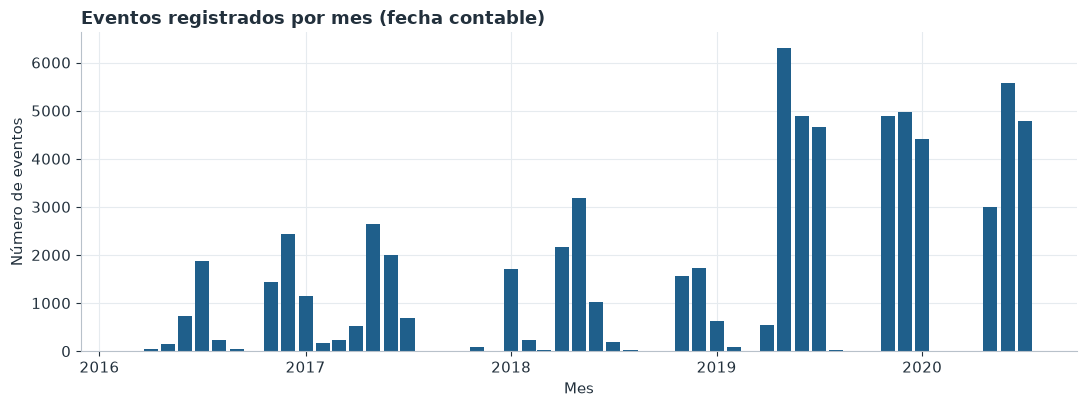
\includegraphics[width=0.92\textwidth]{eventos_por_mes.png}
\caption{Eventos registrados por mes (fecha contable). Los meses vacíos son visibles como huecos.}
\label{fig:eventos}
\end{figure}

Las 177 columnas se clasificaron con reglas automáticas (Tabla~\ref{tab:clasif}). Solo 57 (32.2\,\%) son cuantitativas; el resto son identificadores, atributos de calendario y categorías heredadas de tablas de dimensión. La distinción discreta/continua se hizo por regla, por lo que algunas medidas redondeadas (por ejemplo \texttt{TONELADA\_DECLARADA}, \texttt{LATITUD} y \texttt{LONGITUD}) quedaron como discretas aunque miden magnitudes continuas.

\begin{table}[h!]
\centering
\caption{Clasificación automática de las 177 columnas}
\label{tab:clasif}
\begin{tabular}{llrl}
\toprule
\textbf{Naturaleza} & \textbf{Subtipo} & \textbf{Columnas} & \textbf{Ejemplos} \\
\midrule
Cuantitativa & Continua            & 38 & \texttt{TO}, \texttt{TED}, \texttt{TONELADA\_REAL} \\
Cuantitativa & Discreta            & 19 & \texttt{NUMERO\_CALAS\_CFO}, \texttt{CAPACIDAD\_BODEGA} \\
Cualitativa  & Ordinal             & 30 & \texttt{RANGO\_FAENAS}, \texttt{TRIMESTRE} \\
Cualitativa  & Nominal             & 27 & \texttt{CENTRO\_ZONA\_PESCA}, \texttt{NOMBRE\_FLOTILLA} \\
Cualitativa  & Identificador/código & 25 & \texttt{Row\_ID}, \texttt{EMBARCACION\_ID} \\
Cualitativa  & Binaria             & 19 & \texttt{RSW\_PROCESO}, \texttt{CUOTA\_PROPIA} \\
Temporal     & Fecha/hora          & 19 & \texttt{FECHA}, \texttt{FECHA\_FIN\_DESCARGA} \\
\bottomrule
\end{tabular}
\end{table}

% ===================================================================
\section{Criterios de tabla ordenada (tidy)}
% ===================================================================

Se evaluaron nueve criterios con evidencia calculada sobre los datos (Tabla~\ref{tab:tidy}): tres se cumplen, tres se cumplen parcialmente y tres no se cumplen. La única llave primaria confiable es \texttt{Row\_ID}; las llaves de negocio candidatas (por ejemplo embarcación más fecha contable) tienen decenas de miles de filas en grupos repetidos.

\begin{table}[h!]
\centering
\caption{Resultado del checklist de tabla ordenada}
\label{tab:tidy}
\begin{tabular}{p{4.6cm}lp{7.2cm}}
\toprule
\textbf{Criterio} & \textbf{Estado} & \textbf{Evidencia principal} \\
\midrule
Sin filas vacías & Cumple & 0 filas totalmente vacías. \\
Sin columnas vacías & Parcial & 0 columnas vacías, pero 1 con más de 90\,\% de nulos. \\
Una sola fila de encabezado & Parcial & Un encabezado, pero 8 nombres de columna duplicados. \\
Sin totales o subtotales & Cumple & 0 celdas con texto de total o suma. \\
Fechas en un solo formato & No cumple & 19 columnas temporales con 5 representaciones distintas. \\
Cada variable en una columna & No cumple & Bloque \texttt{*\_PLAN}, 16 columnas \texttt{*\_IND}, 8 duplicadas (\texttt{.1}) y calidad repartida en 3 columnas. \\
Sin obstrucciones & Parcial & Sin celdas combinadas, pero 258\,917 celdas de texto con espacios sobrantes. \\
Una unidad observacional por tabla & No cumple & El evento se mezcla con atributos de embarcación, temporada y flotilla. \\
Llave primaria & Cumple & \texttt{Row\_ID} es único; las llaves naturales no. \\
\bottomrule
\end{tabular}
\end{table}

% ===================================================================
\section{Datos faltantes}
% ===================================================================

Solo 61 de las 177 columnas están completas y \texttt{CAUSA\_NO\_PESCA\_ID} llega a 96.1\,\% de nulos (Figura~\ref{fig:nulos}). El hallazgo más importante es que el archivo no contiene celdas vacías: los nulos vienen como el texto \texttt{NULL} (2\,453\,974 celdas, típico de una exportación SQL) y existen además \textbf{faltantes disfrazados} (Tabla~\ref{tab:disfrazados}).

\begin{figure}[h!]
\centering
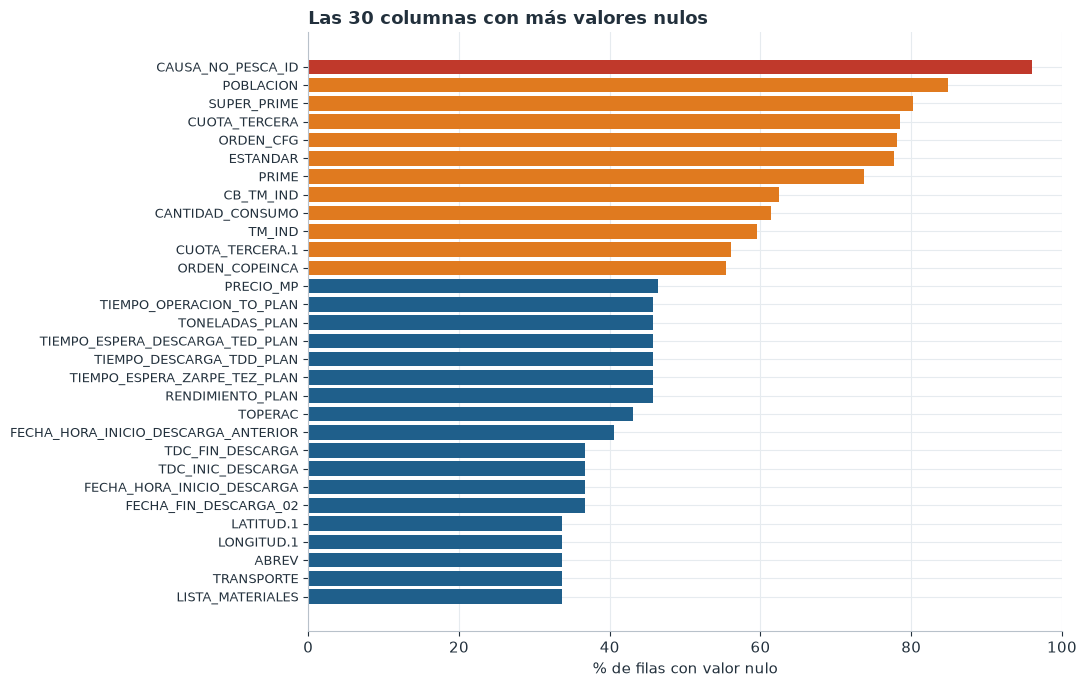
\includegraphics[width=0.88\textwidth]{nulos_top30.png}
\caption{Las 30 columnas con mayor porcentaje de nulos (rojo: más de 90\,\%; naranja: 50--90\,\%).}
\label{fig:nulos}
\end{figure}

\begin{table}[h!]
\centering
\caption{Faltantes disfrazados detectados}
\label{tab:disfrazados}
\begin{tabular}{lr}
\toprule
\textbf{Valor} & \textbf{Ocurrencias} \\
\midrule
Texto \texttt{NULL} (nulos reales) & 2\,453\,974 \\
\texttt{SIN DATOS} & 100\,324 \\
Celdas en blanco & 69\,632 \\
\texttt{\#VALUE!} (error de hoja de cálculo) & 23\,577 \\
Coordenadas 0/0 & 2\,790 \\
Fecha centinela \texttt{19000101} & 38 \\
\bottomrule
\end{tabular}
\end{table}

Los nulos no son aleatorios: 25 columnas faltan a la vez en 33.2\,\% de las filas (eventos sin descarga) y el bloque \texttt{*\_PLAN} falta completo en 45.7\,\% de las filas.

% ===================================================================
\section{Valores atípicos}
% ===================================================================

Se aplicaron el criterio del rango intercuartílico (1.5$\times$IQR) y el z robusto (umbral 3.5), además de reglas de lógica de negocio. Las duraciones \texttt{TO}, \texttt{TED} y \texttt{TEZ} alcanzan valores cercanos al millón (máximos de 1\,028\,846, 1\,042\,048 y 1\,025\,474) frente a medianas de 17.7 y 2.3 en \texttt{TO} y \texttt{TED}; 406 valores superan 720 (un mes si la unidad fueran horas, aunque la unidad exacta se desconoce). Además, 4\,104 descargas superan la capacidad de la bodega y 74 posiciones válidas caen fuera de la costa peruana, con longitudes de hasta $-98.2$ (Figura~\ref{fig:coord}).

\begin{figure}[h!]
\centering
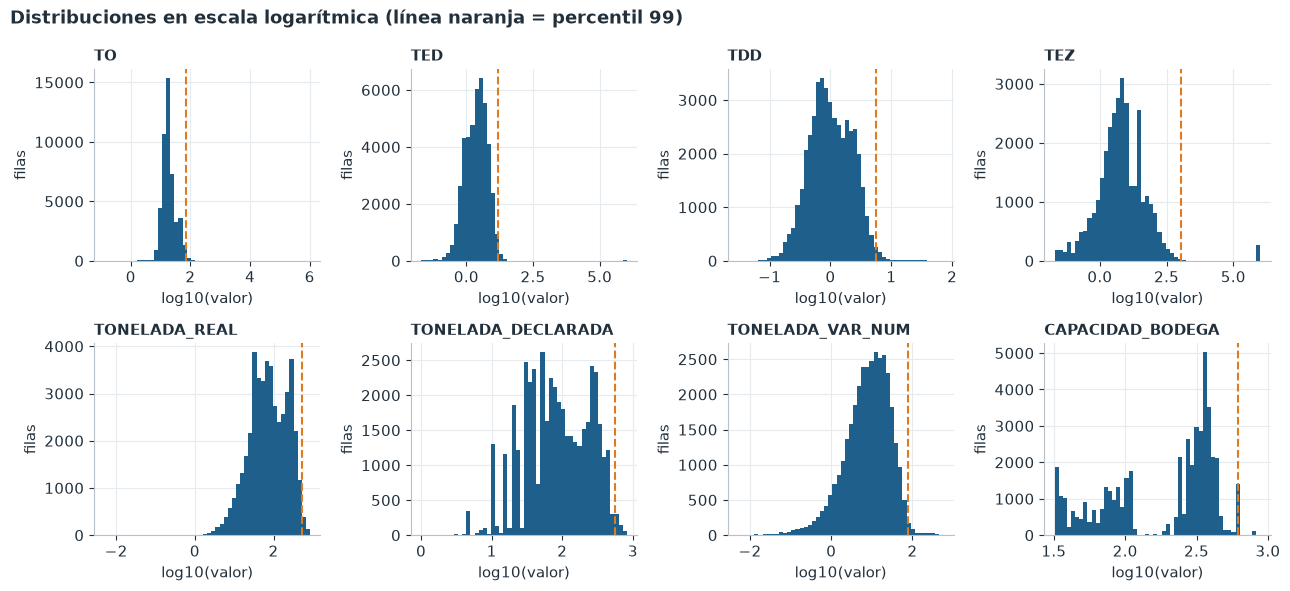
\includegraphics[width=0.95\textwidth]{distribuciones_log.png}
\caption{Distribuciones en escala logarítmica de las variables clave; la línea naranja marca el percentil 99.}
\label{fig:dist}
\end{figure}

\begin{figure}[h!]
\centering
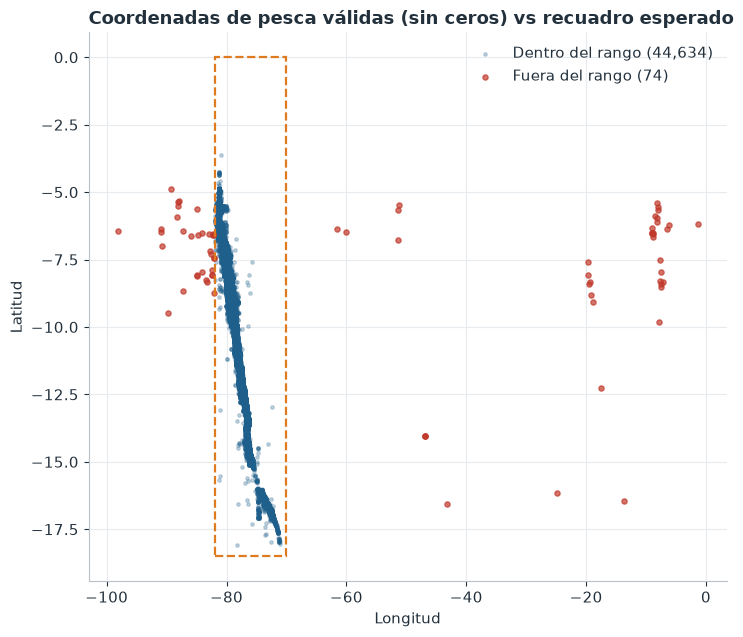
\includegraphics[width=0.62\textwidth]{coordenadas.png}
\caption{Coordenadas de pesca válidas frente al recuadro esperado para el litoral peruano.}
\label{fig:coord}
\end{figure}

% ===================================================================
\section{Valores únicos y cálculos derivados}
% ===================================================================

\begin{itemize}
  \item \textbf{Constantes:} 15 columnas tienen un solo valor y no aportan información.
  \item \textbf{Códigos numéricos:} 24 columnas numéricas son en realidad códigos y no deben promediarse.
  \item \textbf{Categorías casi iguales:} aparecen variantes como \texttt{FLOTILA} y \texttt{FLOTILLA}.
  \item \textbf{Columnas duplicadas:} 7 grupos de columnas (16 en total) tienen contenido idéntico; en los pares \texttt{.1} de una misma variable no hay conflictos.
  \item \textbf{\texttt{TONELADA\_VAR}:} donde es numérica, coincide en el 100\,\% de las 47\,498 filas comparables con \texttt{TONELADA\_DECLARADA} $-$ \texttt{TONELADA\_REAL}, es decir, con signo contrario al que sugiere su nombre. Sus 23\,577 valores no numéricos son todos \texttt{\#VALUE!}.
  \item \textbf{Capacidad de bodega:} difiere entre columnas equivalentes en 18\,248 filas.
\end{itemize}

% ===================================================================
\section{Catálogo de casuísticas}
% ===================================================================

Cada hallazgo se registró con las columnas involucradas, las filas afectadas y una severidad. La Tabla~\ref{tab:cat} y la Figura~\ref{fig:cat} resumen las 51 casuísticas por categoría; el detalle completo está en el notebook.

\begin{table}[h!]
\centering
\caption{Casuísticas por categoría y severidad}
\label{tab:cat}
\begin{tabular}{lrrrr}
\toprule
\textbf{Categoría} & \textbf{Total} & \textbf{Alta} & \textbf{Media} & \textbf{Baja} \\
\midrule
Consistencia & 9 & 3 & 5 & 1 \\
Outliers     & 5 & 3 & 2 & 0 \\
Centinela    & 9 & 2 & 5 & 2 \\
Faltantes    & 4 & 2 & 2 & 0 \\
Formato      & 9 & 1 & 5 & 3 \\
Estructura   & 5 & 1 & 3 & 1 \\
Privacidad   & 1 & 1 & 0 & 0 \\
Duplicidad   & 4 & 0 & 4 & 0 \\
Constantes   & 3 & 0 & 0 & 3 \\
Categorías   & 1 & 0 & 0 & 1 \\
Temporal     & 1 & 0 & 0 & 1 \\
\midrule
\textbf{Total} & \textbf{51} & \textbf{13} & \textbf{26} & \textbf{12} \\
\bottomrule
\end{tabular}
\end{table}

\begin{figure}[h!]
\centering
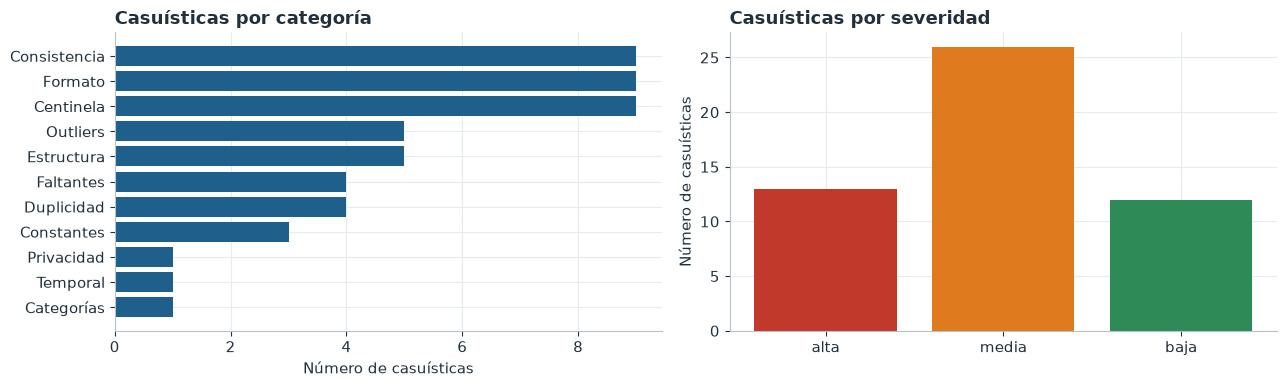
\includegraphics[width=0.95\textwidth]{casuisticas_resumen.png}
\caption{Casuísticas por categoría y por severidad.}
\label{fig:cat}
\end{figure}

% ===================================================================
\section{Lectura desde las dimensiones de calidad}
% ===================================================================

La Tabla~\ref{tab:dim} ordena la evidencia según las dimensiones clásicas de calidad de datos. Es una \textbf{lectura del perfilado, no un veredicto}: afirmar que los datos son de calidad requiere reglas y umbrales de negocio que este trabajo no define. La oportunidad (qué tan actual es el dato) no se evalúa porque se desconoce la fecha de extracción.

\begin{table}[h!]
\centering
\caption{Dimensiones de calidad según la evidencia del perfilado}
\label{tab:dim}
\begin{tabular}{lp{8.3cm}p{2.8cm}}
\toprule
\textbf{Dimensión} & \textbf{Evidencia} & \textbf{Lectura} \\
\midrule
Completitud  & 19.5\,\% de las celdas son nulas; solo 61 de 177 columnas completas; 12 columnas con más de 50\,\% de nulos. & Baja \\
Validez      & 16 fechas \texttt{19000101}, 2\,790 filas con coordenada 0 y formatos de fecha mezclados. & Débil \\
Exactitud    & 4\,104 descargas sobre la capacidad de la bodega, 406 duraciones sobre 720 y 74 posiciones fuera de la costa. & Dudosa (sin fuente externa no se confirma) \\
Unicidad     & 0 filas duplicadas y 0 \texttt{Row\_ID} repetidos, pero 15 columnas constantes y 7 grupos de columnas idénticas. & Buena en filas, débil en columnas \\
Consistencia & \texttt{TONELADA\_VAR} con signo contrario al del nombre y capacidad de bodega distinta entre columnas en 18\,248 filas. & Débil \\
\bottomrule
\end{tabular}
\end{table}

% ===================================================================
\section{Conclusiones}
% ===================================================================

\begin{itemize}
  \item El archivo es una tabla de hechos de 71\,075 eventos que aplana varias dimensiones (embarcación, temporada, flotilla, calendario); solo 57 de sus 177 columnas son realmente cuantitativas.
  \item Los faltantes son en gran parte estructurales (eventos sin descarga) y están disfrazados como texto (\texttt{NULL}, \texttt{SIN DATOS}, \texttt{\#VALUE!}), por lo que no se detectan con una revisión superficial.
  \item Existen valores centinela y valores extremos en fechas, coordenadas y duraciones que distorsionarían cualquier análisis posterior si no se identifican.
  \item Se catalogaron 51 casuísticas en 11 categorías (13 de severidad alta); el perfilado señala calidad baja en completitud, validez y consistencia, y deja la exactitud como dudosa a falta de una fuente de contraste.
  \item Varias interpretaciones (unidad de \texttt{TO} y \texttt{TED}, significado de las columnas \texttt{TDC\_*}, posibles vedas) son hipótesis que deben validarse con el área de negocio.
\end{itemize}

\end{document}
